\documentclass{article}
\usepackage{amsmath}
\usepackage{graphicx}

\title{CS 461 Homework 1}
\author{Mannan Shukla}
\date{Due: Sept. 27, 11:59 pm}

\begin{document}

\maketitle

\section*{Problem 1: Right Choice for Empirical Metric}

\subsection*{1.1 Precision Rate}
Precision Rate measures the rate of positive values that are in the classification
circle. The formula is

\[
\frac{\text{\# of observed positive examples}}{\text{\# of samples in the circle}}
\]

The classification circle trained on this data would be a small circle surrounding
1 positive example. This would ensure a precision rate of 100\%.

\subsection*{1.2 Recall Rate}
Recall Rate measures the rate of observed positive values by the total number
of positive values in the dataset. The formula is

\[
\frac{\text{\# of observed positive examples}}{\text{\# of total positive examples}}
\]

The classification circle trained on this data would be huge. In fact, it would
classify the entire dataset to make sure that no positive values are left behind.

\subsection*{1.3 Issues and Suggested Metric}
The main issue with using precision rate as the only metric for classification
is that it’s very easy to miss a lot of data since the classification circle would
be so small to ensure a 100\% rate. The opposite is true of recall rate. Since
it would be focused on maximizing the total amount of positive examples, the
circle would be too big and it would take in 5 negative examples to take 1
positive one. The precision rate for such a classification would be horrible.

The solution is to strike a balance between the two. You could use the F1
score, which is just the harmonic mean between precision rate and recall rate.

\[
F1 = 2 \cdot \frac{\text{precision} \cdot \text{recall}}{\text{precision} + \text{recall}}
\]

\section*{Problem 2: Galton Board}

\subsection*{2.1 Sample Spaces Definition}
Since the ball only has the choice between moving left and right at each level,
we can define $\Omega_M = \{L, R\}$. The choice is the same from $\Omega_2 \dots \Omega_M$.

\subsection*{2.2 Sample Space Representation}
$\Omega$ is the cartesian product of all of the subspaces $\Omega_2 \dots \Omega_M$. We can use the
following set builder notation to define:

\[
\Omega = \{(x_1, x_2, \dots, x_M) \ | \ x_i \in \{L, R\}, i \in \mathbb{Z}, 1 \le i \le M\}
\]

\subsection*{2.3 Meaning of the Location at $L_G$}
The meaning of $L_G$, where the ball arrives, is simply the number of right turns
the ball took. $L_G$ defines the place or bin where the ball ends up, which is
dictated by the number of right turns.

\subsection*{2.4 Numerical Representation of Location}
We can define $L_G$ as the random variable $X$. Since there are only two possibilities
with an equal probability $p = 0.5$, we can use the following binomial distribution
to describe the distribution:

\[
P(X = k) = \binom{M}{k}\left(\frac{1}{2}\right)^M
\]

\subsection*{2.5 PMF of the Random Variable and Central Limit Theorem}
Define the PMF of your random variable for depths $M = 5$, $M = 10$, and
$M = 100$. Plot them and explain the phenomenon in relation to the Central
Limit Theorem.

\subsection*{Central Limit Theorem (CLT) Explanation}
The Central Limit Theorem (CLT) states that the distribution of the sum (or
average) of independent random variables, each with finite mean and variance,
approaches a normal distribution as the number of variables increases. In the
context of the Galton board, as the number of levels $M$ increases, the binomial
distribution for the number of successes $k$ begins to approximate a normal
distribution. We can see that visually in the following figure:

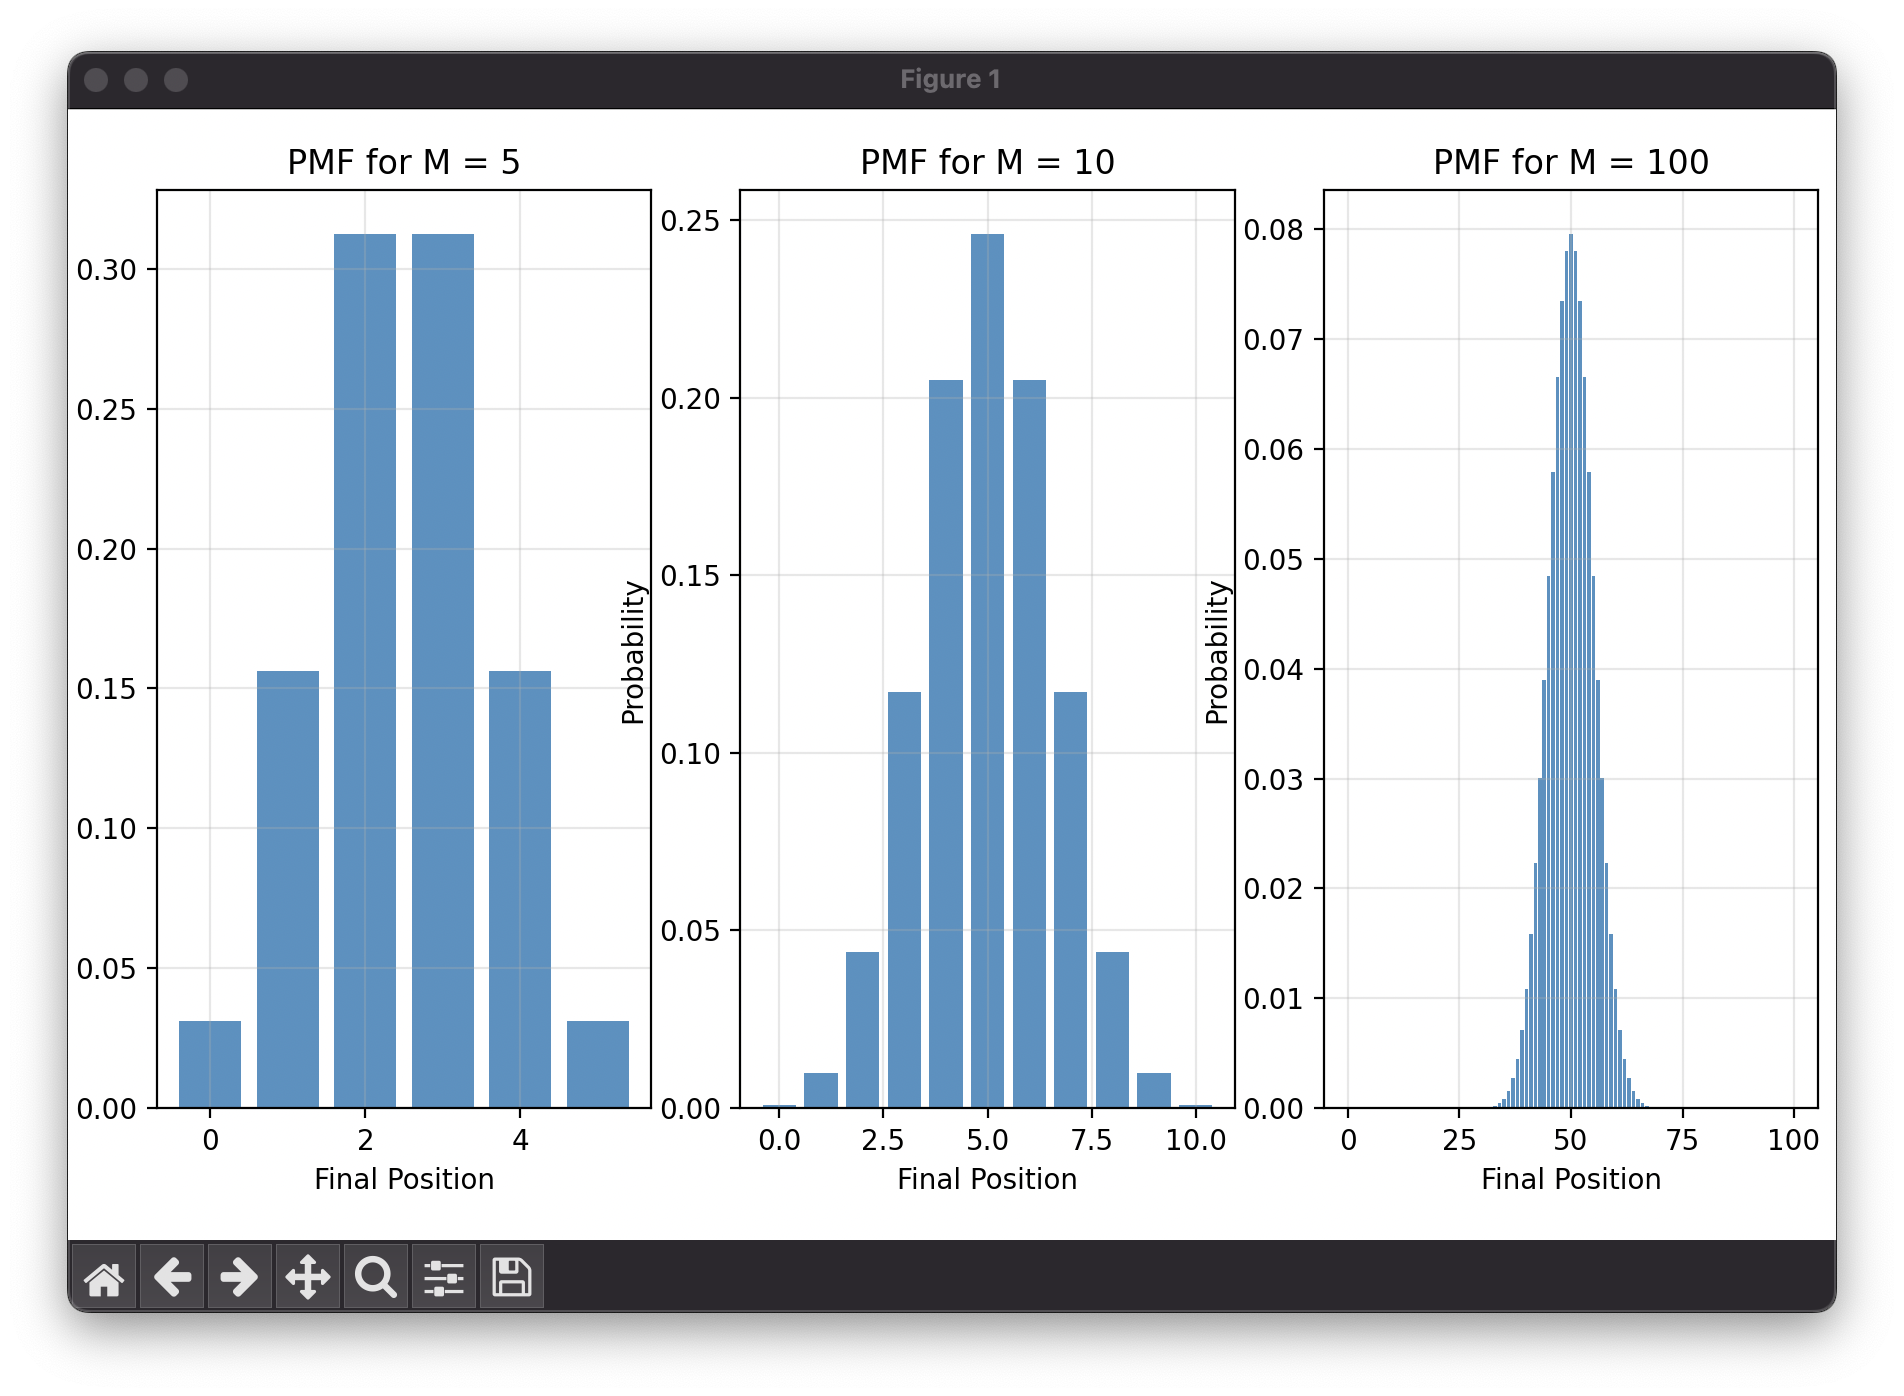
\includegraphics[width=\linewidth]{clt.png}

\section*{Problem 3: Bayes Rule}

\subsection*{3.1 Probability of Survival}
We want to calculate $P(D)$. Given:

\[
P(D|F) = 0.8, \quad P(D|F') = 0.2, \quad P(F) = 0.3
\]

We can find $P(F') = 1 - P(F) = 0.7$. Now, using marginalization:

\[
P(D) = P(D,F) + P(D,F') = (P(D|F) \cdot P(F)) + (P(D|F') \cdot P(F'))
\]

\[
P(D) = (0.8 \cdot 0.3) + (0.2 \cdot 0.7) = 0.38
\]

Thus, the probability that the plant survives is:

\[
P(D') = 1 - P(D) = 0.62
\]

\subsection*{3.2 Probability if Friend Forgot to Water}
This is simply:
\[
P(D|F) = 0.8
\]

\subsection*{3.3 Probability that Friend Forgot to Water Based on Death}
Using Bayes’ theorem:

\[
P(F|D) = \frac{P(D|F) \cdot P(F)}{P(D)} = \frac{0.8 \cdot 0.3}{0.38} = 0.6316
\]

\section*{Problem 4: Naive Bayes}

\subsection*{4.1 Formula Rewrite for Naive Bayes}
$P(D = +|G = g,B = b) = \frac{P(G=g|D=+)\cdot P(B=b|D=+)\cdot P(D=+)}{(P(G=g|D=+)\cdot P(B=b|D=+)\cdot P(D=+))+(P(G=g|D=-)\cdot P(B=b|D=-)\cdot P(D=-))} \\ \\ P(D = -|G = g,B = b) = \frac{P(G=g|D=-)\cdot P(B=b|D=-)\cdot P(D=-)}{(P(G=g|D=+)\cdot P(B=b|D=+)\cdot P(D=+))+(P(G=g|D=-)\cdot P(B=b|D=-)\cdot P(D=-))}$

\subsection*{4.2 Estimation Based on Train Data}
Look at \texttt{mannan-nb-train.py}

\subsection*{4.3 Classifier Code}
Look at \texttt{mannan-nb-cls.py}

\subsection*{4.4 Evaluation of Classifier}
Look at \texttt{mannan-nb-test.py}

\subsection*{4.5 Standardization Necessity}
Standardization is not really helpful for Naive Bayes classification. For Gaussian
Naive Bayes, we are just looking at the mean and variance. These metrics aren’t
affected by scaling or standardization, so it isn’t needed for this classifier.

\subsection*{4.6 Data Reflection and Improvements}
The dataset may not fully capture real-world diabetes diagnoses since it only
includes glucose and blood pressure, while other factors like age or BMI are
also important. There could also be biases if the data comes from a limited
population. Without new data, feature engineering, such as creating a glucose-
to-blood-pressure ratio, and using cross-validation could improve the model’s
accuracy and generalizability.

\section*{Problem 5: Data Whitening}

\subsection*{5.1 Expressing $E[Y]$ and COV[$Y, Y$]}
Let $Y = A \cdot X + b$, where $A$ is a transformation matrix and $b$ is a bias vector.
The expected value of $Y$ is:

\[
E[Y] = A \cdot E[X] + b
\]

Given $E[X] = \begin{bmatrix} 0.2 \\ 0.3 \\ 0.1 \end{bmatrix}$, we have:

\[
E[Y] = A \cdot \begin{bmatrix} 0.2 \\ 0.3 \\ 0.1 \end{bmatrix} + b
\]

The covariance matrix of $Y$ is:

\[
\text{COV}[Y, Y] = A \cdot \text{COV}[X, X] \cdot A^T
\]

Given the covariance matrix $\text{COV}[X, X] = \begin{bmatrix} 2.75 & 0.43 & 0 \\ 0.43 & 2.25 & 0 \\ 0 & 0 & 1 \end{bmatrix}$, the covariance
of $Y$ becomes:

\[
\text{COV}[Y, Y] = A \cdot \begin{bmatrix} 2.75 & 0.43 & 0 \\ 0.43 & 2.25 & 0 \\ 0 & 0 & 1 \end{bmatrix} \cdot A^T
\]

\subsection*{5.2 Design A and b for Whitening}
To whiten the data, we need to set $E[Y] = 0$ and $\text{COV}[Y, Y] = I$.
\begin{enumerate}
    \item Setting $E[Y] = 0$: \\
    The expected value of $Y$ is:

    \[
    E[Y] = A \cdot E[X] + b
    \]

    To achieve $E[Y] = 0$, we set:

    \[
    b = -A \cdot E[X]
    \]

    Thus, the calculated $b$ is:

    \[
    b = \begin{bmatrix} -0.1052 \\ -0.1912 \\ -0.1 \end{bmatrix}
    \]

    \item Setting $\text{COV}[Y, Y] = I$: \\
    The covariance of $Y$ is:

    \[
    \text{COV}[Y, Y] = A \cdot \text{COV}[X, X] \cdot A^T
    \]

    We want $\text{COV}[Y, Y] = I$, which leads to the equation:

    \[
    A \cdot \text{COV}[X, X] \cdot A^T = I
    \]

    Therefore, the transformation matrix $A$ is the inverse square root of the
    covariance matrix $\text{COV}[X, X]$. The calculated $A$ is:

    \[
    A = \begin{bmatrix} 0.6097 & -0.0558 & 0 \\ -0.0558 & 0.6746 & 0 \\ 0 & 0 & 1 \end{bmatrix}
    \]
\end{enumerate}

\section*{Problem 6: ML and MAP Estimation}

\subsection*{6.1 Maximum Likelihood Estimate (MLE)}
Given that the observations $x_1, x_2, \dots, x_n$ are i.i.d. and follow a Gaussian distribution, the probability density function for each observation $x_i$ is:

\[
f(x_i|\mu, \sigma^2) = \frac{1}{\sqrt{2\pi\sigma^2}} \exp\left(- \frac{(x_i - \mu)^2}{2\sigma^2}\right)
\]

The likelihood function for all observations is the product of the individual probabilities, and the log-likelihood is:

\[
\log L(\mu, \sigma^2) = -\frac{n}{2} \log(2\pi\sigma^2) - \frac{1}{2\sigma^2} \sum_{i=1}^{n} (x_i - \mu)^2
\]

To find the MLE for $\mu$, we differentiate the log-likelihood with respect to $\mu$
and set it to zero:

\[
\frac{d}{d\mu} \log L(\mu, \sigma^2) = \frac{1}{\sigma^2} \sum_{i=1}^{n} (x_i - \mu) = 0
\]

Solving for $\mu$, we obtain the MLE:

\[
\mu^* = \frac{1}{n} \sum_{i=1}^{n} x_i
\]

\subsection*{6.2 Maximum A Posteriori (MAP) Estimate}
Let $X_1, \dots, X_N$ be i.i.d. random variables with a PDF:

\[
f_{X_n|\mu}(x_n|\mu) = \frac{1}{\sqrt{2\pi\sigma^2}} \exp\left(- \frac{(x_n - \mu)^2}{2\sigma^2}\right)
\]

and let $\mu$ have a prior distribution:

\[
f_\mu(\mu) = \frac{1}{\sqrt{2\pi\sigma_0^2}} \exp\left(- \frac{(\mu - \mu_0)^2}{2\sigma_0^2}\right)
\]

The MAP estimate is:

\[
\hat{\mu}_{MAP} = \arg\max_\mu p(\mu|x) \propto p(x|\mu) \cdot p(\mu)
\]

Taking the logarithm of the likelihood and prior:

\[
\hat{\mu}_{MAP} = \arg\max_\mu \left\{-\frac{1}{2\sigma^2} \sum_{n=1}^{N} (x_n - \mu)^2 - \frac{(\mu - \mu_0)^2}{2\sigma_0^2}\right\}
\]

Differentiating with respect to $\mu$:

\[
\sum_{n=1}^{N} \frac{(x_n - \mu)}{\sigma^2} - \frac{(\mu - \mu_0)}{\sigma_0^2} = 0
\]

Solving for $\mu$, we get:

\[
\mu \left(\frac{N}{\sigma^2} + \frac{1}{\sigma_0^2}\right) = \frac{\sum_{n=1}^{N} x_n}{\sigma^2} + \frac{\mu_0}{\sigma_0^2}
\]

The final MAP estimate is:

\[
\hat{\mu}_{MAP} = \frac{\sum_{n=1}^{N} x_n \cdot \sigma_0^2 + \mu_0 \cdot \sigma^2}{N\sigma_0^2 + \sigma^2}
\]

\subsection*{6.3 Behavior of MAP for $N \to \infty$ and $N \to 0$}
The MAP estimate is:

\[
\mu_{MAP} = \frac{\sigma^2}{N\sigma_0^2 + \sigma^2} \mu_0 + \frac{N\sigma_0^2}{N\sigma_0^2 + \sigma^2} \mu_{ML}
\]

\begin{itemize}
    \item As $N \to \infty$: The prior $\mu_0$ loses influence, so $\mu_{MAP} \to \mu_{ML}$.
    \[
    \lim_{N \to \infty} \mu_{MAP} = \mu_{ML}
    \]
    \item As $N \to 0$: The data loses influence, so $\mu_{MAP} \to \mu_0$.
    \[
    \lim_{N \to 0} \mu_{MAP} = \mu_0
    \]
\end{itemize}

In short, use MLE when $N$ is large and MAP when $N$ is small.

\end{document}
